\section{System Design}
\label{sec:system_design} %%for reference in other section

%% image reference : \ref{fig:circle_project}
%%\begin{figure}
%%	\centering    	
%%\includegraphics[width=0.90\textwidth,natwidth=610,natheight=642]{figs/xxx.jpg}
%%  	\caption{Kickstarter Project: Meet Circle}
%%  	\label{fig:circle_project}
%%\end{figure}

%% list
%%\begin{itemize}
%%  	\item Strict development time (and runtime) enforcement of module boundaries
%%	\item ...
%%  \end{itemize}

%% table reference : \ref{tab:improve_system_func}
%% \begin{table}
%% \caption{\label{tab:improve_system_func}: Improvement Functions for System}
%% \centering
%% \begin{tabular}{| c | p{4cm} | p{6cm} | l |}
%% \hline
%% No. & Title & Improvement Function & Importance \\ \hline
%% 1 & Block Internet Access & The residential access point can block clients internet access base on MAC and forbid the \gls{ip} address request & High \\ \hline
%% 2 & Bug Fixed for static \gls{ip} lease & Bug found in the report with wrong script format in static \gls{ip} lease for residential access point & High \\ \hline
%% \end{tabular} 
%% \end{table}

%% bibliography reference
%% \cite{xxx}

\par At the design and preparation stage one important thing should be taken into an account. System need to be highly flexible and able to dynamically adapt to changing requirements. Self-adaptive system was taken as a base. After that, we decide to make this project working for big range of different services in the smart house scope by making the complicated central management and easy client devices architecture. The main architecture of the system is shown in Figure \ref{fig:system_architecture}.
Sources for the project can be found in the internet by the address %%https://github.com/pavelArteev/ttm3_osgi_smartHouse.git.
\begin{figure}
	\centering    	
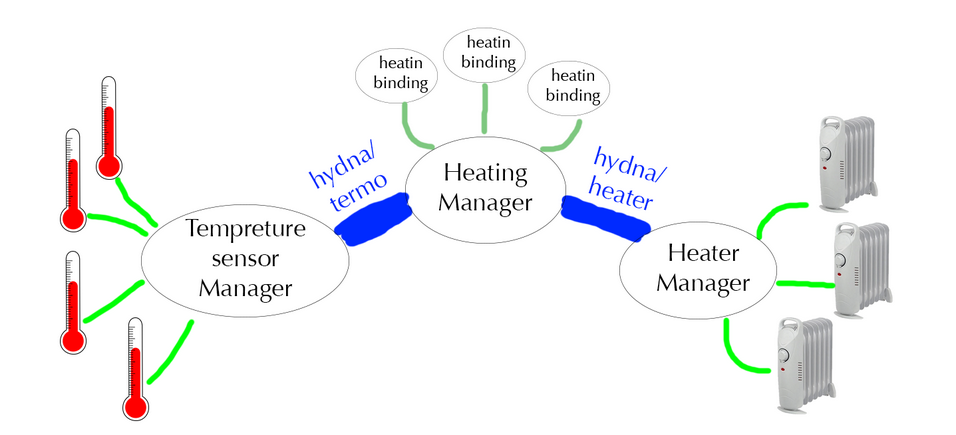
\includegraphics[width=0.90\textwidth,natwidth=610,natheight=642]{figs/system_architecture.png}
  	\caption{Smart Heating System Architecture}
  	\label{fig:system_architecture}
\end{figure}

\subsection{Temperature Sensor Manager}
\par Temperature Sensor Manager is a service to provide control command to temperature sensor and observe temperature sensor client. In this prototype project it is included in the Heater Simulator OSGi bundle.  In this prototype it has an user friendly control panel to demonstrate the temperature sensor client changes. In the normal use case it should communicate with other 'stupid' temperature sensor in some local communication channel, like Zigbee, Bluetooth or Radio Frequency. The main functions of temperature sensor manager are to get the raw data from the temperature sensor (in prototype project which is only string type data) and to send these raw data to the Heating Manager through remote communication channel (Hydna backend service in this project, channel domain: ithouse.hydna.net/thermometer) and listen to this communication channel to wait for heating manager control command if necessary. That means the local communication channel and remote communication channel both have two way function to work with in the system. In the prototype project, there is a user friendly user interface to simulate the temperature changes through slide the slides in the control panel of temperature simulator. The working application is shown in the Figure \ref{fig:sensor_simulators} with the user interface slide label 'Tempreture'. Once the sliding the slide to demonstrate the temperature changes in the real work then temperature sensor manager will send message with format in Code Snippet\ref{code:message_format}. Then the central heating manager will decide if it need to send message to notify binding heater to turn on or turn off. In this whole process all the device clients have only one basic functionality based on what kind of device they are. This architecture of the system make other service could be possible to reuse it by just changing different OSGi service bundle in the system, which is the key point of our project.

\begin{algorithm}[h]
\floatname{algorithm}{Code Snippet}
  \caption{Hydna Message Format}
  \label{code:message_format}
  \begin{verbatim}
  <hydna message type> : <message source> : <message destination> : <message command>
 \end{verbatim}
\end{algorithm}

\begin{figure}
	\centering    	
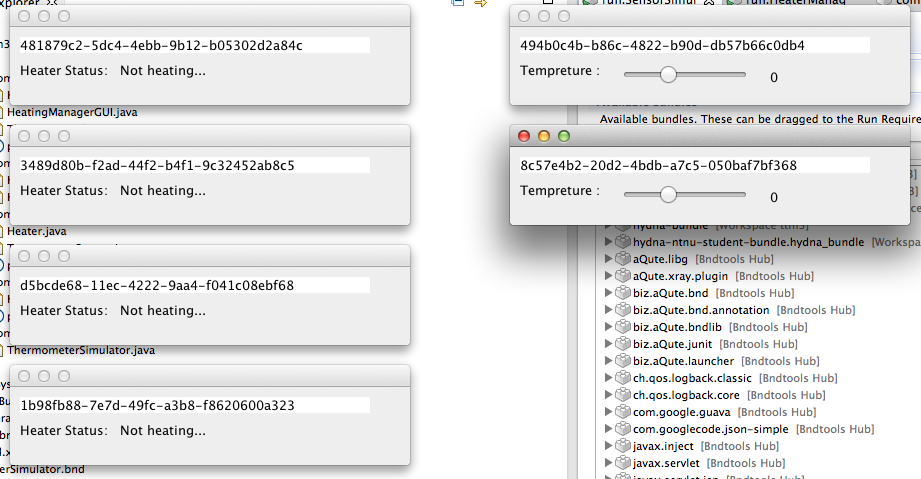
\includegraphics[width=0.90\textwidth,natwidth=610,natheight=642]{figs/sensor_simulators.png}
  	\caption{Smart Heating System Sensor Simulators}
  	\label{fig:sensor_simulators}
\end{figure}

\clearpage

\begin{algorithm}[h]
\floatname{algorithm}{Code Snippet}
  \caption{processMessage function in Heater Manager}
  \label{code:heater_process_message}
  \begin{verbatim}
  // Message  type:src:dst:cmd
	private void processMessage(String message){
		String[] strArray = {};
		strArray = message.split(":");
		if(strArray.length<4){
			return;
		}else{
			String msgType = strArray[0];
			String msgSrc = strArray[1];
			String msgDst = strArray[2];
			String msgCmd = strArray[3];
			// trying to process message
			if(msgType.equals(Heater.SERVER_MESSAGE)){
				//find address in array
				HeaterSimulatorItem hsi = heaterMap.get(msgDst);
				if(hsi!=null){
					if(msgCmd.equals(Heater.CMD_STATUS)){
						hydnaSvc.sendMessage(Heater.CLIENT_MESSAGE 
							+ ":" + msgDst + ":" 
							+ msgSrc + ":" 
							+ Heater.CMD_STATUS 
							+ "@" + hsi.getHeater().getStatus());
					}else if(msgCmd.equals(Heater.CMD_HEATER_ON)){
						hsi.getGUI().startHeating();
						hsi.getHeater().setHeat(true);
						hydnaSvc.sendMessage(Heater.CLIENT_MESSAGE 
							+ ":" + msgDst + ":" 
							+ msgSrc + ":" 
							+ Heater.CMD_STATUS 
							+ "@" + hsi.getHeater().getStatus());
					}else if(msgCmd.equals(Heater.CMD_HEATER_OFF)){
						hsi.getGUI().stopHeating();
						hsi.getHeater().setHeat(false);
						hydnaSvc.sendMessage(Heater.CLIENT_MESSAGE + ":" 
							+ msgDst + ":" 
							+ msgSrc + ":" 
							+ Heater.CMD_STATUS 
							+ "@" + hsi.getHeater().getStatus());
					}
				}
			}else if(msgType.equals(Heater.CLIENT_MESSAGE)){
				// Ignore this
			}
		}
		
	}
 \end{verbatim}
\end{algorithm}

\subsection{Heater Manager}
\par Heater Manager is a similar service as Temperature Sensor Manager to provide bridge between Heating Manager and heater devices. In our prototype project, it is included in Heater Simulator OSGi bundle as well. The running application of it is shown in the Figure \ref{fig:sensor_simulators} with the user interface label 'Heater Status'. The different between Heater Manager service and Temperature Sensor Manager service is that Heater Manager need to listen to another Hydna  remote communication channel(channel domain: ithouse.hydna.net/heater) to get the correct control command to responsible heater device. Once it get the control command from the Heating Manager then it will understand what kind of command it is then make the corresponding heater device working correctly according to the command. For the goal of simplifying the project message in the Hydna, in this  project we are using the same message format in Code Snippet \ref{code:message_format}, only with the different hyena message type and message command content. The code to provide the function of processing message got from Heating Manager is shown in the Code Snippet \ref{code:heater_process_message}. The function works based on not only the control command but also the current status of the corresponding  heater device. Then in this system, again the manager service takes care of the 'dump' device clients and device clients only care about basic function of them. This mechanism make the boundaries between the different service component in the system, that's the key part of the self-component system to separate the different services in different component to reduce the dependence of each other. By OSGi, we can easily install and upgrade some service bundle in the system later to make some improvement of the system or replace with other service. 

\subsection{Heating Manager}
\par Heating Manager is the core of the whole system. It provides the logic to bind the different temperature sensor and heater device as an useful working service for the user and also provide the control logic by the message from temperature sensors and heater device clients. In our prototype project, there is an user interface as well which is shown in Figure \ref{fig:heating_manager}. There are four initial services user interface allocated for the purpose of demonstration. By typing the UUID in the text box in the user interface, then the corresponding heater and temperature sensor will be bind as a user heating service. There are a threshold slides bar in the service which can be controlled by the user to set the ideally temperature of the room or house. Then the Heating Manager will do the working process according to the system algorithm which is shown in Figure \ref{fig:system_algorithm}, it will trigger some control message if necessary then send it to the Hydna remote communication channel(if control message is for heater, most case, the channel domain will be: ithouse.hydna.net/heater) with the same message format in Code Snippet \ref{code:message_format}. Then the Heater Manager will get the message to do the command to corresponding heater device. Since the Heating Manager need to observe the temperature data in 'thermometer'(channel domain: ithouse.hydna.net/thermometer) channel and heater manager connection status in 'heater' (channel domain: ithouse.hydna.net/heater)channel, then we implemented these listener in different thread to avoid the conflict between different message event in different channel. But at first there is no getinstance function in provided hydna-ntnu-student-bundle\cite{hydna_ntnu_student_bundle}, then we make our own generateNewApiInstance method in the hydna-ntnu-student-bundle. It provides resources to run the api service in different Java thread, it is a fast way to get the multiple thread solution but maybe not the best way.

\begin{figure}
	\centering    	
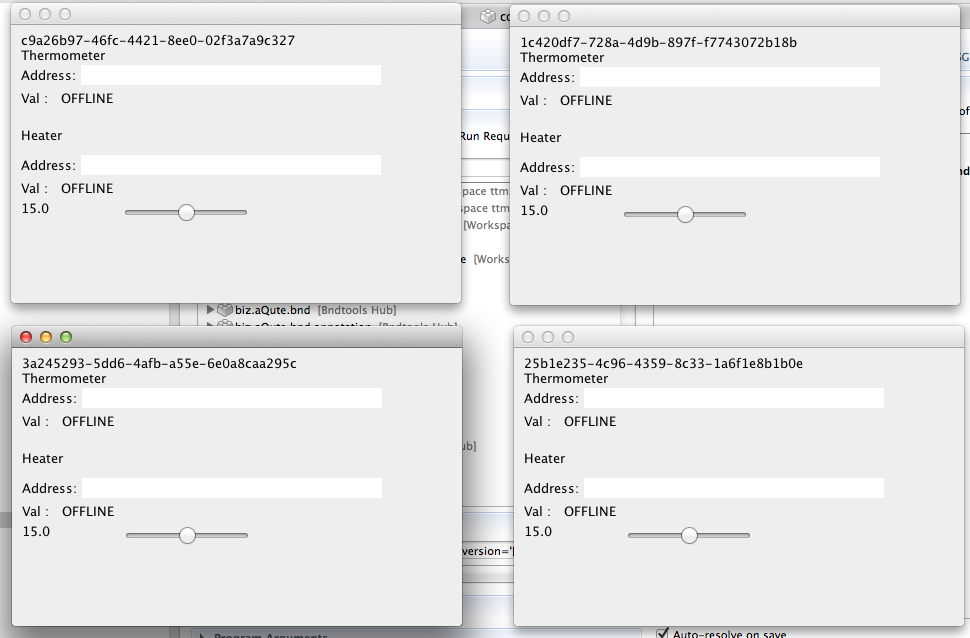
\includegraphics[width=0.90\textwidth,natwidth=610,natheight=642]{figs/heating_manager.png}
  	\caption{Smart Heating System Heating Manager GUI}
  	\label{fig:heating_manager}
\end{figure}

\clearpage

\begin{figure}
	\centering    	
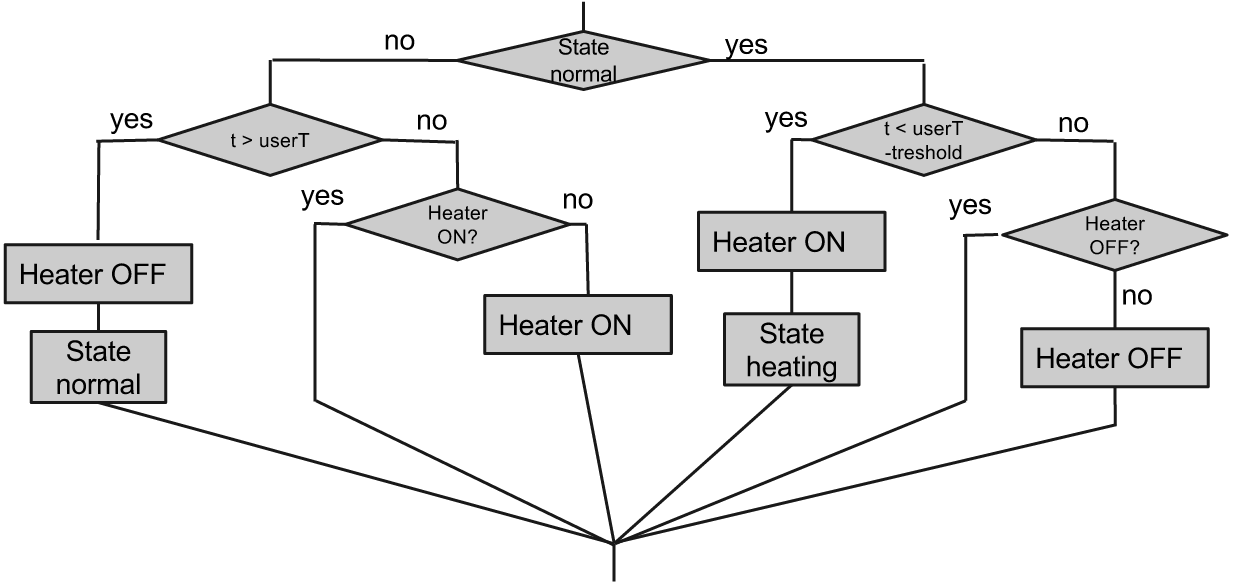
\includegraphics[width=0.90\textwidth,natwidth=610,natheight=642]{figs/system_algorithm.png}
  	\caption{Smart Heating System Heating Manager Algorithm}
  	\label{fig:system_algorithm}
\end{figure}

\par In the system algorithm shown in Figure \ref{fig:system_algorithm}, it showed that there are two states for each heater, one is state normal, the other is state heating. The state machine implement method helps this system to be simple and flexible with other services later as well. In the Heating Manager service bundle, it just needs to ask for the current state of the heater then according to the message of the temperature sensor and user configured threshold to send control command to the Heater Manager. Heating Manager just need to make sure if the communication between itself and remote communication channel working well. When the Heater Manager is offline for some reason, then the binding service will be trashed by Heating Manager, the only notification is from remote Hydna 'heater' channel.


